\documentclass[9pt,twocolumn]{paper-template}
% Use the lineno option to display guide line numbers if required.

\usepackage{lipsum}
\templatetype{twocolumn} % Choose template 
% {pnasresearcharticle} = Template for a two-column research article
% {pnasmathematics} %= Template for a one-column mathematics article
% {pnasinvited} %= Template for a PNAS invited submission

\title{Temporal Neural Analysis on Motor Cortex}

% Use letters for affiliations, numbers to show equal authorship (if applicable) and to indicate the corresponding author
\author[a]{Mahdi Norouzi}
\author[a]{Arsalan Firoozi}

\affil[a]{Bachelor Student, Electrical Engineering Department, Sharif University of Technology}

% Keywords are not mandatory, but authors are strongly encouraged to provide them. If provided, please include two to five keywords, separated by the pipe symbol, e.g:
\keywords{Temporal $|$ Motor $|$ Neural Coding} 

\begin{abstract}
Using recorded motor neuron's data of a macaque monkey during a reach-to-grasp task, we studied how motor and premotor neural responses are related to events in time. Our hypothesis is that motor neurons are activated during the monkey's hand movements and features such as force and direction are encoded in activation pattern. This study shows that activation during hand movements can be acceptable and some movement features are encoded in these neurons.
\end{abstract}

\dates{This manuscript was compiled on \today}

\begin{document}

\maketitle
\thispagestyle{firststyle}
\ifthenelse{\boolean{shortarticle}}{\ifthenelse{\boolean{singlecolumn}}{\abscontentformatted}{\abscontent}}{}

% If your first paragraph (i.e. with the \dropcap) contains a list environment (quote, quotation, theorem, definition, enumerate, itemize...), the line after the list may have some extra indentation. If this is the case, add \parshape=0 to the end of the list environment.
\dropcap{B}ody movement involves a range of complex actions, especially in primates. Over the years, different regions of the cortex have been associated with motor actions, which are three areas of the frontal lobe: the premotor cortex, primary motor cortex, and supplementary motor area. Moreover, a substantial amount of studies has turned their attention to hand movements. Various aspects and parameters, such as speed, force, direction, etc., contribute to this unique motion.
\\
Until now, the majority of research has focused on the spatial tuning of movement-related areas. However, there hasn’t been sufficient evidence regarding the temporal responses of the motor cortex and the role of individual neurons in coding movement parameters. On the one hand, it is not clear that there need be any straightforward relationship between neural responses and movement parameters. Meanwhile, some studies have shown a simple relationship between the measured responses of motor cortex neurons and kinematic parameters like reach direction and speed. (1)
\\
We have addressed these issues by analyzing electrophysiological recordings made during a delayed reach-to-grasp task from the motor cortex of a male macaque monkey. This experiment is done in four types of tasks, different in direction and force of grasp. Each task consists of a handful of events that have been manually timestamped and allow us to investigate neural responses concerning the time of these events. Also, through examining single neuron activities in each type of grasp, we inspect the notion of aspects like force and direction, being coded by individual neurons. All these analyses are done by statistical testing on two key features, extracted from spike trains; firing rate and Fano factor.
 
\section*{Materials and Methods}
The dataset used in this paper is made available by the German Neuroinformatics Node of the International Neuroinformatics Coordination Facility (INCF). It contains recordings from the motor cortex with a 10-by-10 Utah electrode array during controlled reach-to-grasp movements for two macaque monkeys (L and N) and the data that we used for our analysis was gathered only from the right hemisphere of monkey N, the male monkey. The Utah array was surgically implanted a few millimeters anterior to the central sulcus, aimed to be located in the arm/hand representation of the primary motor cortex with the most anterior electrodes encroaching upon the premotor cortex. Particularly in monkey N, the array encompassed two areas; M1 and the premotor ventral cortex (PMv).\\
\begin{figure}%[tbhp]
\centering
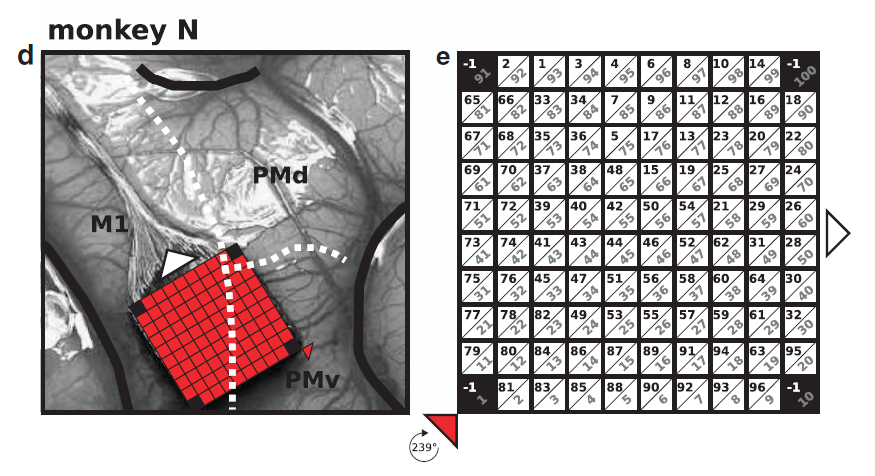
\includegraphics[width=.8\linewidth]{fig1.PNG}
\caption{The left picture shows the orientation of the implanted array regarding the wire bundle (white triangle) and the picture to the right indicates its default orientation. Also in the picture of the implanted array, M1 and PMv areas can be distinctly recognized by the putative border (the vertical dotted line). These pictures were provided in the source paper of the dataset material. (2) }
\label{fig:frog}
\end{figure}
\\
After leaving out the four inactive corner cells of the array, each of the 96 recorded neural signals was differentially amplified and filtered with a 1st-order 0.3 Hz high pass filter (full-bandwidth mode) and a 3rd-order 7.5 kHz Butterworth low pass filter. The band-pass filtered neuronal signals were digitized with 16-bit resolution at 0.25 V/bit and a sampling rate of 30 kHz, in the following called “raw signal”. Then the LFP data was extracted from a copy of the raw data, digitally low-pass filtered at 250 Hz (Butterworth, 4th order), and down sampled to 1 kHz. Furthermore, by filtering and sorting different combinations of the raw signal through waveform detection, 271 different spike trains have been obtained which represent different neural masses, including single and multiple unit activities. To investigate neurons individually, we concentrated our analyses only on the 156 single unit activities (SUAs).
\\
In the task provided by the monkey, he had to grasp the object using either a side grip (SG) or a precision grip (PG) and then pull the object towards him against one of two possible loads requiring either a high or low pulling force (HF and LF, respectively); finally, he would have received the maximum reward if he had pulled the object in the correct grasp for at list 500 ms. The mixture of these experiments leads to four types of task, allowing us to examine on the direction and force of grasp. This experiment was orchestrated by exactly time distanced digital instruction signals given to the monkey through different LED combinations. Each signal represented a specific event initiated from the control system in LabVIEW. Also, there were some events initiated by the monkey recorded through digital or analog signals, representing his movements and interaction with the object.
\\
\begin{figure}%[tbhp]
\centering
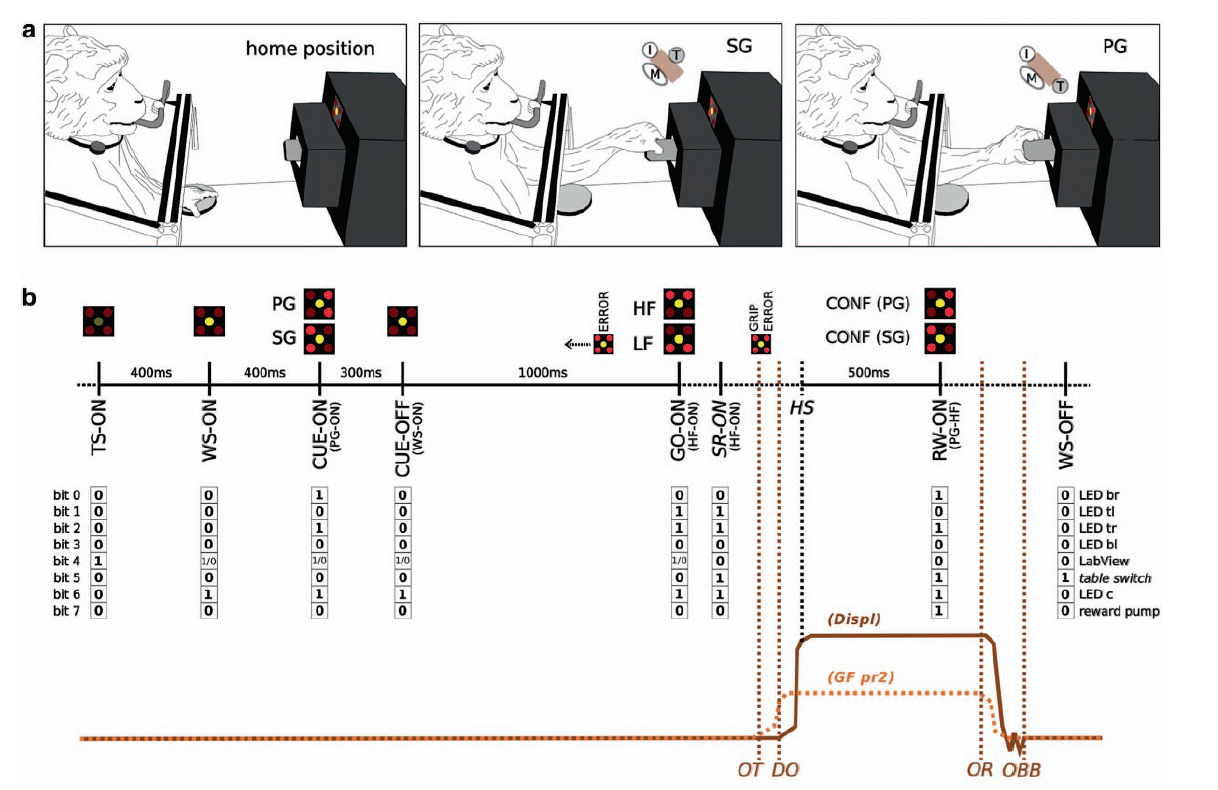
\includegraphics[width=.8\linewidth]{fig2.PNG}
\caption{ Events and their chronological orders. The first event is TS-ON, which is only internally set by LabVIEW to mark the start of the trial. After that, the monkey receives three signals: WS-ON, CUE-ON and GO, subsequently to warn him of the trial start, give him the grasp direction and to signal the movement start (also giving him the required force type). SR event, marks the time he has lifted his hand from the rest position switch and is going to reach the object. RW-ON and STOP(WS-OFF) happen respectively after the monkey has pulled the object for the required duration, and to mark the end of the trial. These pictures were provided in the source paper of the dataset material. (2)}
\label{fig:frog}
\end{figure}
\\
For monkey N, the recording day lasted for one hour with the dataset i140703-001 as first out of 3 recording sessions in the late morning. The recording session of monkey N lasted 16:43 min in which they performed 160 trials. However, he successfully completed 90\% of all trials during the recording and performed 19 error trials, which consisted of 16 grip type errors and 3 early movement initiation errors. According to the dataset paper, the four different tasks were distributed equally so that after removing the error trials we would be left with almost the same number of correct trials for each task.\\
\begin{table}%[tbhp]
\centering
\caption{Number of errors and correct trials}
\begin{tabular}{lrrr}
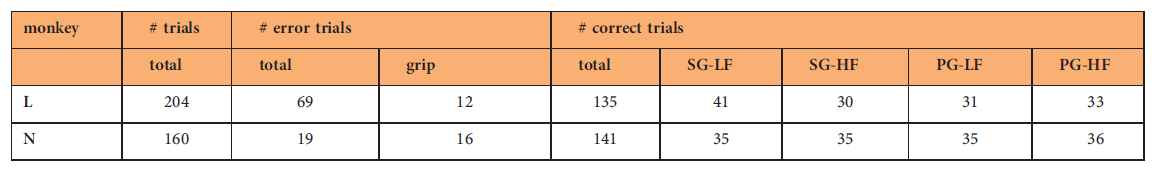
\includegraphics[width=1\linewidth]{fig3.PNG}
\end{tabular}

\addtabletext{These pictures were provided in the source paper of the dataset material. (2)}
\end{table}
\\
We extracted the spike trains representing SUAs, by choosing the ones with the 'an\_sua' flag in the dataset. We also removed the error trials based on their recorded events and whether or not the trial included a reward event. At the end, we gathered 142 trials (one error trial was undetected) for each of the 156 single neuron spike trains. In order to analyze each task separately, we categorized the asks into the desired four types by examining the CUE and GO event labels. The result was 35 trails for each LF task and 36 for each of the HFs. Additionally, we separated neurons of the M1 area from the PMv based on their channel IDs, considering the orientation of the implanted array (Which indicates that the array IDs 45,47,49,53,55, and 73 to 94 are located on the PMv).
\\
For analyzing the spike trains, we have used raster plots aligned with the TS-ON event for each of the 156 neurons. These plots show a neuron's spike trains in time domain, from TS-ON to STOP in all trials. But since the timing of events isn't simillar in different trials, in addition to each trial's event times, we have plotted the average timing of events as well.
Along with raster plots, we have plotted a TS-aligned PSTH for each neuron, which is made by the average firing rate (spike/s) of all trials for a single neuron. The firing rates are calculated by moving a rectangular window (binsize = 0.1, moving step = 0.01) in time domain, counting the spikes in each window and dividing the count by the length of the bin.
These raster plots and PSTHs show us the manner, in which the neurons are responding to different events in time-domain.
\\
To quantify and test our hypotheses, firing rate and Fano factor are collected before and after certain events, and averaged on all the neurons. Therefore, we can obtain a distribution of Fano factor and firing rate in different trials and compare them before and after different events. Also we can use their bar plots to check whether the distribution of these features is gausian or not. To test the temporal responses of neurons statistically, T-test is used and p-value is reported. Testing how movement characteristics are coded in motor neurons is done by clustering trials based on direction and force. For each cluster Fano factor and firing rate for SR event are calculated and differences are reported by using PSTH plots.
\section*{Results}
The first piece of information we gathered in our analysis, was the raster plots of each individual neuron. In these plots we could visually examine the changes in firing patterns of each neuron through different trials. As we previously mentioned, each plot is made from stacking spike trains of each trial together and also all of the eight main events and their average times have been marked with a specific color. In the figure below we have chosen the raster plots for four individual neurons, two of which have distinctly different spike patterns.\\
\begin{SCfigure*}[\sidecaptionrelwidth][t]
\centering

\includegraphics[width=13cm]{fig4.jpg}
\caption{Raster plots of single neurons. Each picture shows the raster plot (including 142 correct trials) for one of the chosen neurons, with their index number in the plot title. Note that neuron 123 is part of the PMv area, in contrast to the other three which have been chosen from M1. Event occurrences have been depicted by colored vertical dashes and their average by a vertical line with the same color}\label{fig:side}
\end{SCfigure*}
\\
The next step was extracting PSTH plots for each neuron that could better depict the firing fluctuations. For every neuron we had to separate all the correct trials in time one by one, count the spikes in a moving rectangular window throughout the trial, and finally divide the value of every counted window on its time length (bin size). At the end, the PSTH was made by averaging the firing rates (spike/s) on all of the trials. In the next figure we have shown the PSTH plots for the same four neurons as the previous section and the relevance of each PSTH with its corresponding raster plot is clear.
\\
\begin{SCfigure*}[\sidecaptionrelwidth][t]
\centering

\includegraphics[width=13cm]{fig5.jpg}
\caption{PSTH plots of single neurons. Accordingly, each plot is the PSTH for one of the four chosen neurons. Neuron 123 is located in the PMv area, as opposed to the other three neurons. Average event times have been shown by vertical lines with specific colors. Events in order of occurrence: TS-ON, WS-ON, CUE-ON, CUE-OFF, GO, SR, RW-ON, STOPr}\label{fig:side}
\end{SCfigure*}
\\
For examining the random process pattern in which the neurons were firing, we had to investigate the inter-spike intervals (ISIs) and their distributions. In order to do so, we calculated the differences between spike times of each neuron in throughout   trails, but due to the enormity of the number of available neurons, we decided to gather the ISI distribution for an average neuron by plotting the distribution of all the calculated ISIs together. Additionally, we repeated this procedure by separating neurons of the M1 and PMv areas. The three histogram plots are all shown in the following figure, alongside an exponential distribution with the rate of 25. We can observe that these three plots show similar distributions and all of them can are approximately changing as the same as the exponential pattern (expect for very low ISIs, for which the reason can be insufficient data from the resting position of the specified neurons). This observation could be an indicator that our neurons are firing with the pattern of a Poisson process because it is known that the intervals of an event in the Poisson process follows the exponential distribution.\\
\begin{figure}%[tbhp]
\centering
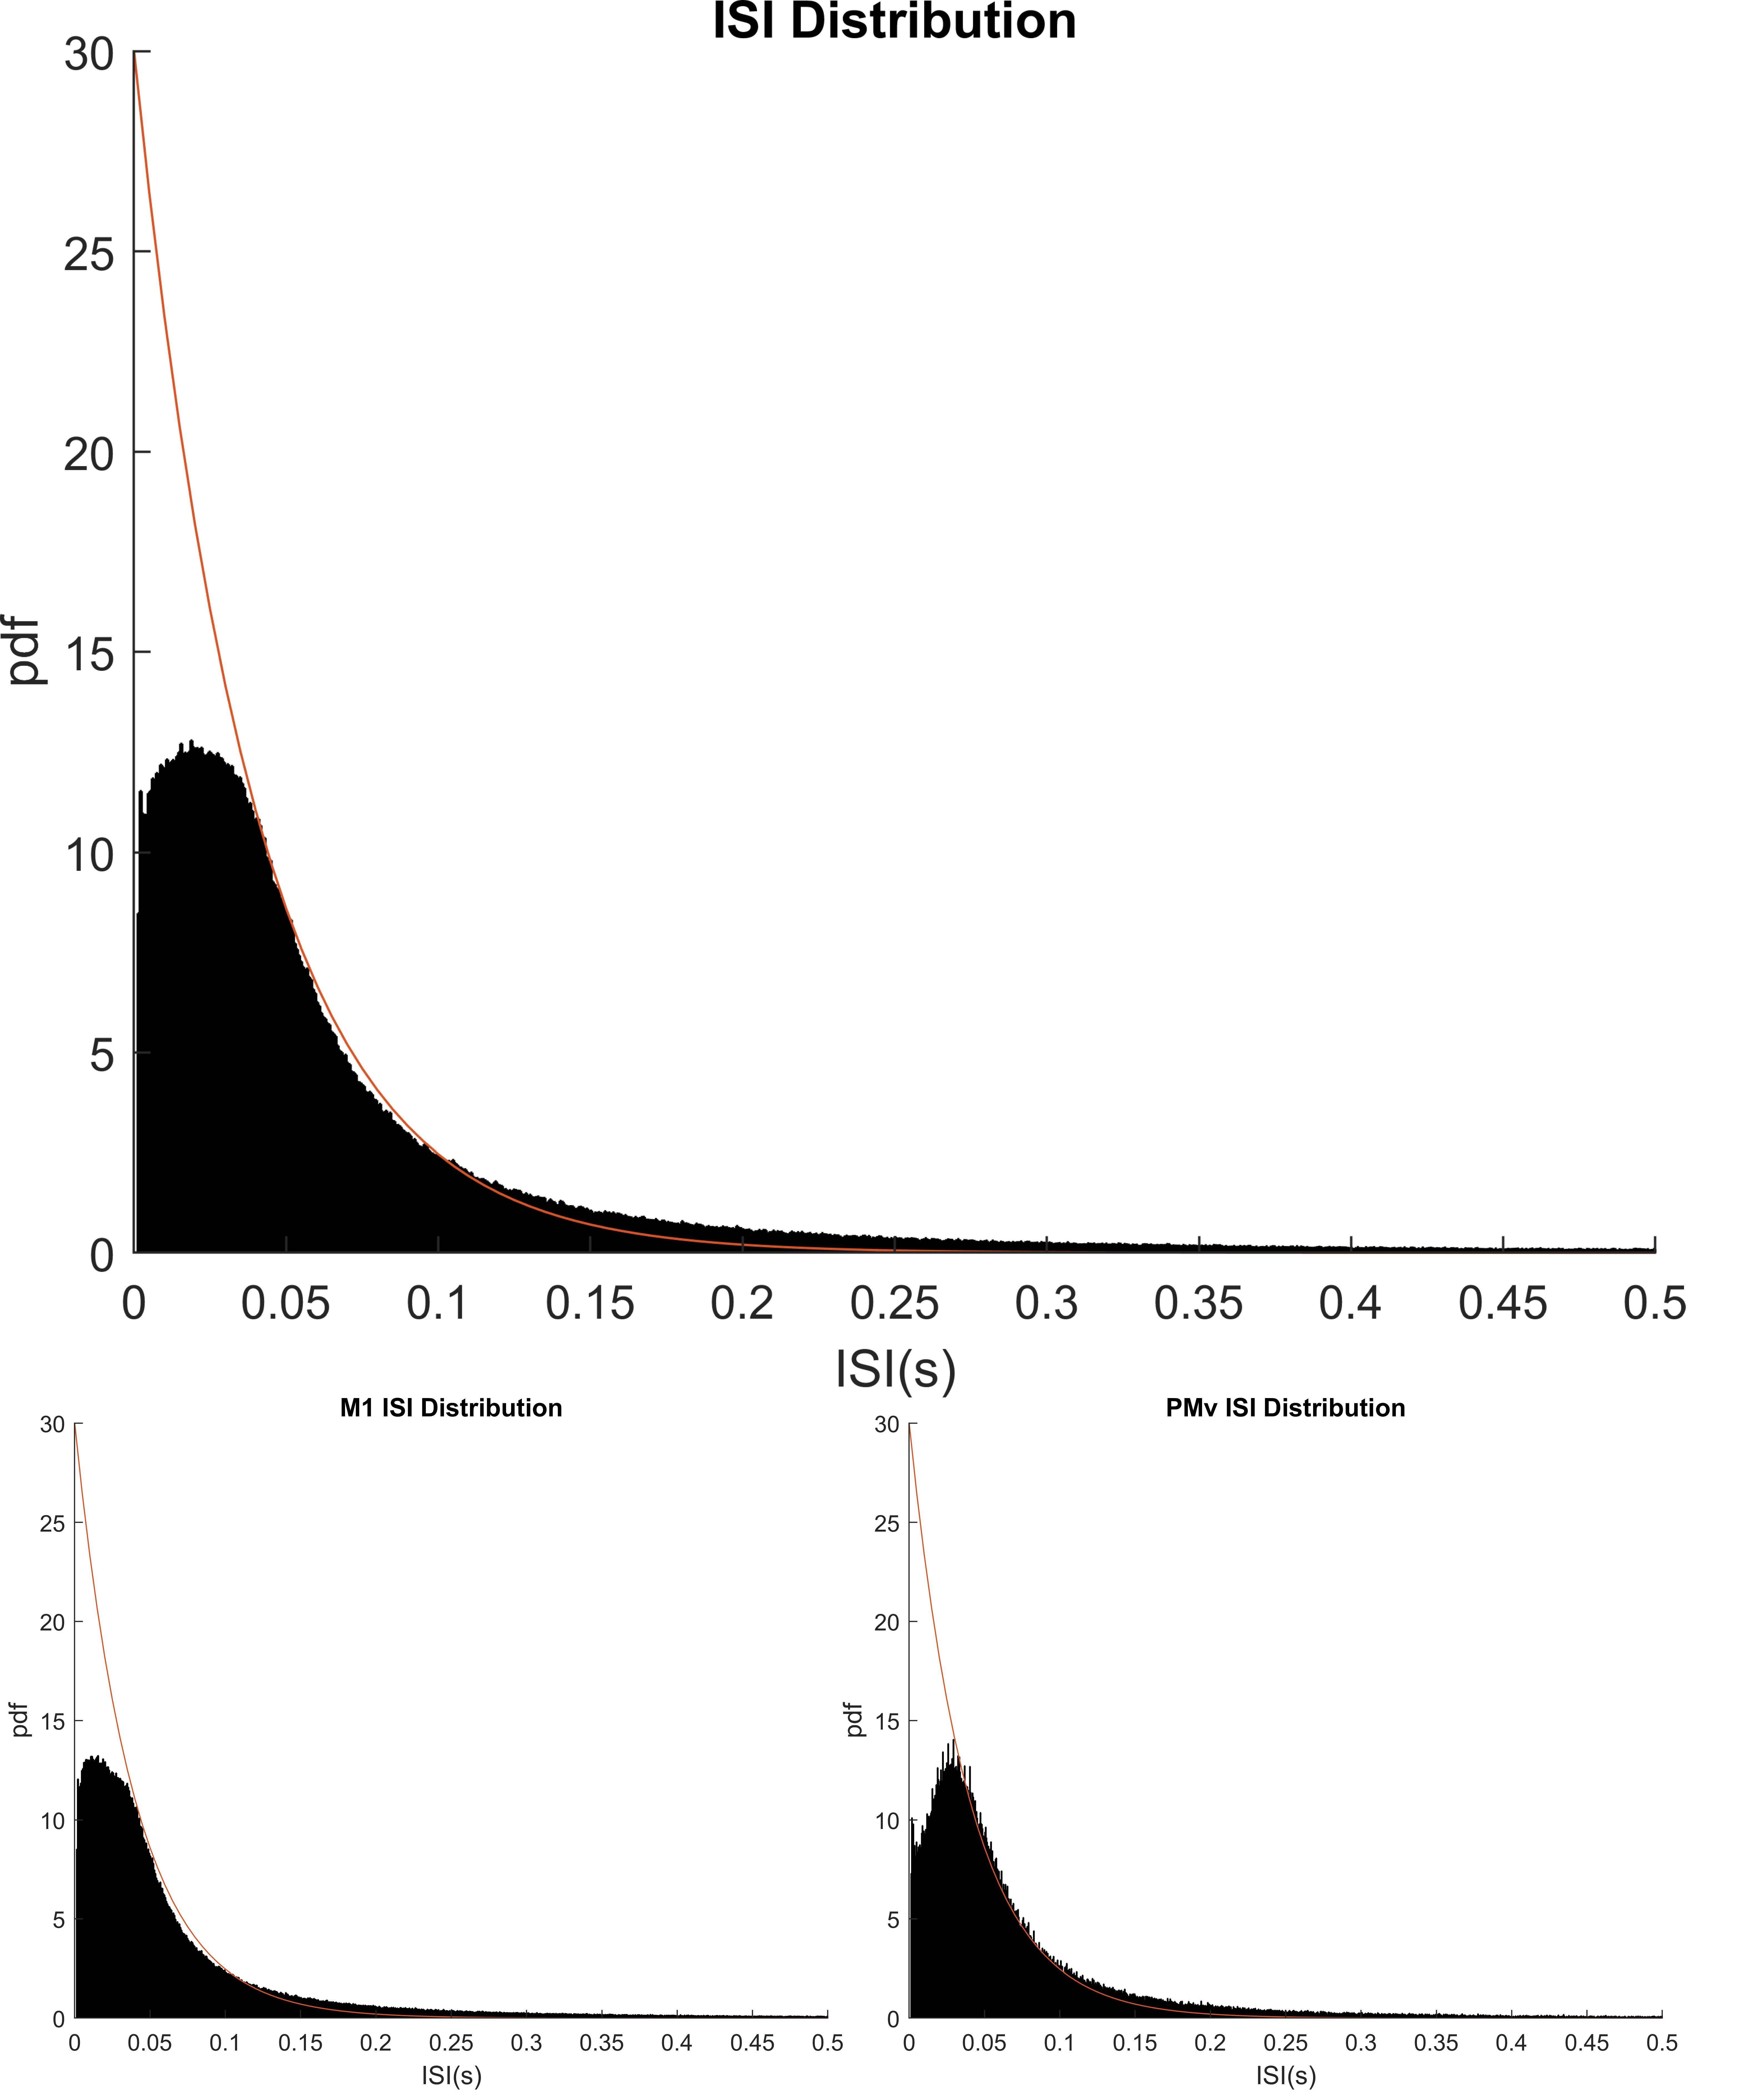
\includegraphics[width=.8\linewidth]{fig6.jpg}
\caption{Average neuron ISI distributions. Each plot shows the histogram of the combined ISIs of a cluster of neurons: all the extracted neurons, neurons from M1, and neurons of the PMv. Additionally, an exponential plot with rate = 25 is shown (red line), alongside the histograms}
\label{fig:frog}
\end{figure}
\\
In order to investigate the temporal correlation between events and firing pattern variations, we had to examine the PSTH plots for individual neurons and seek for signs of event-correspondent changes. However, examining all the 156 single neurons separately was not an option, so once more we decided to obtain an average PSTH response from all neurons and base our hypotheses on that. We also extracted an average PSTH for clusters of M1 and PMv neurons separately. In the PSTH gathered from all neurons, as well as the one attained only from the M1 area, we can see a notable surge in firing rate starting after the GO event and accelerating after SR. It seems reasonable to have an activity increase in the motor area after the initiation signal for movement and during the movement itself. However, in the PMv area, we have a rather high firing rate from the start of the trial leading to a relatively small increase after GO and SR. This could be a confirming evidence of the role known for the premotor cortex to participate in pre-movement planning. Furthermore, we see an abrupt decay of firing rate in all three plots after the RW-ON which can be due to the monkey’s awareness of the end of the trial.
\\
\begin{SCfigure*}[\sidecaptionrelwidth][t]
\centering
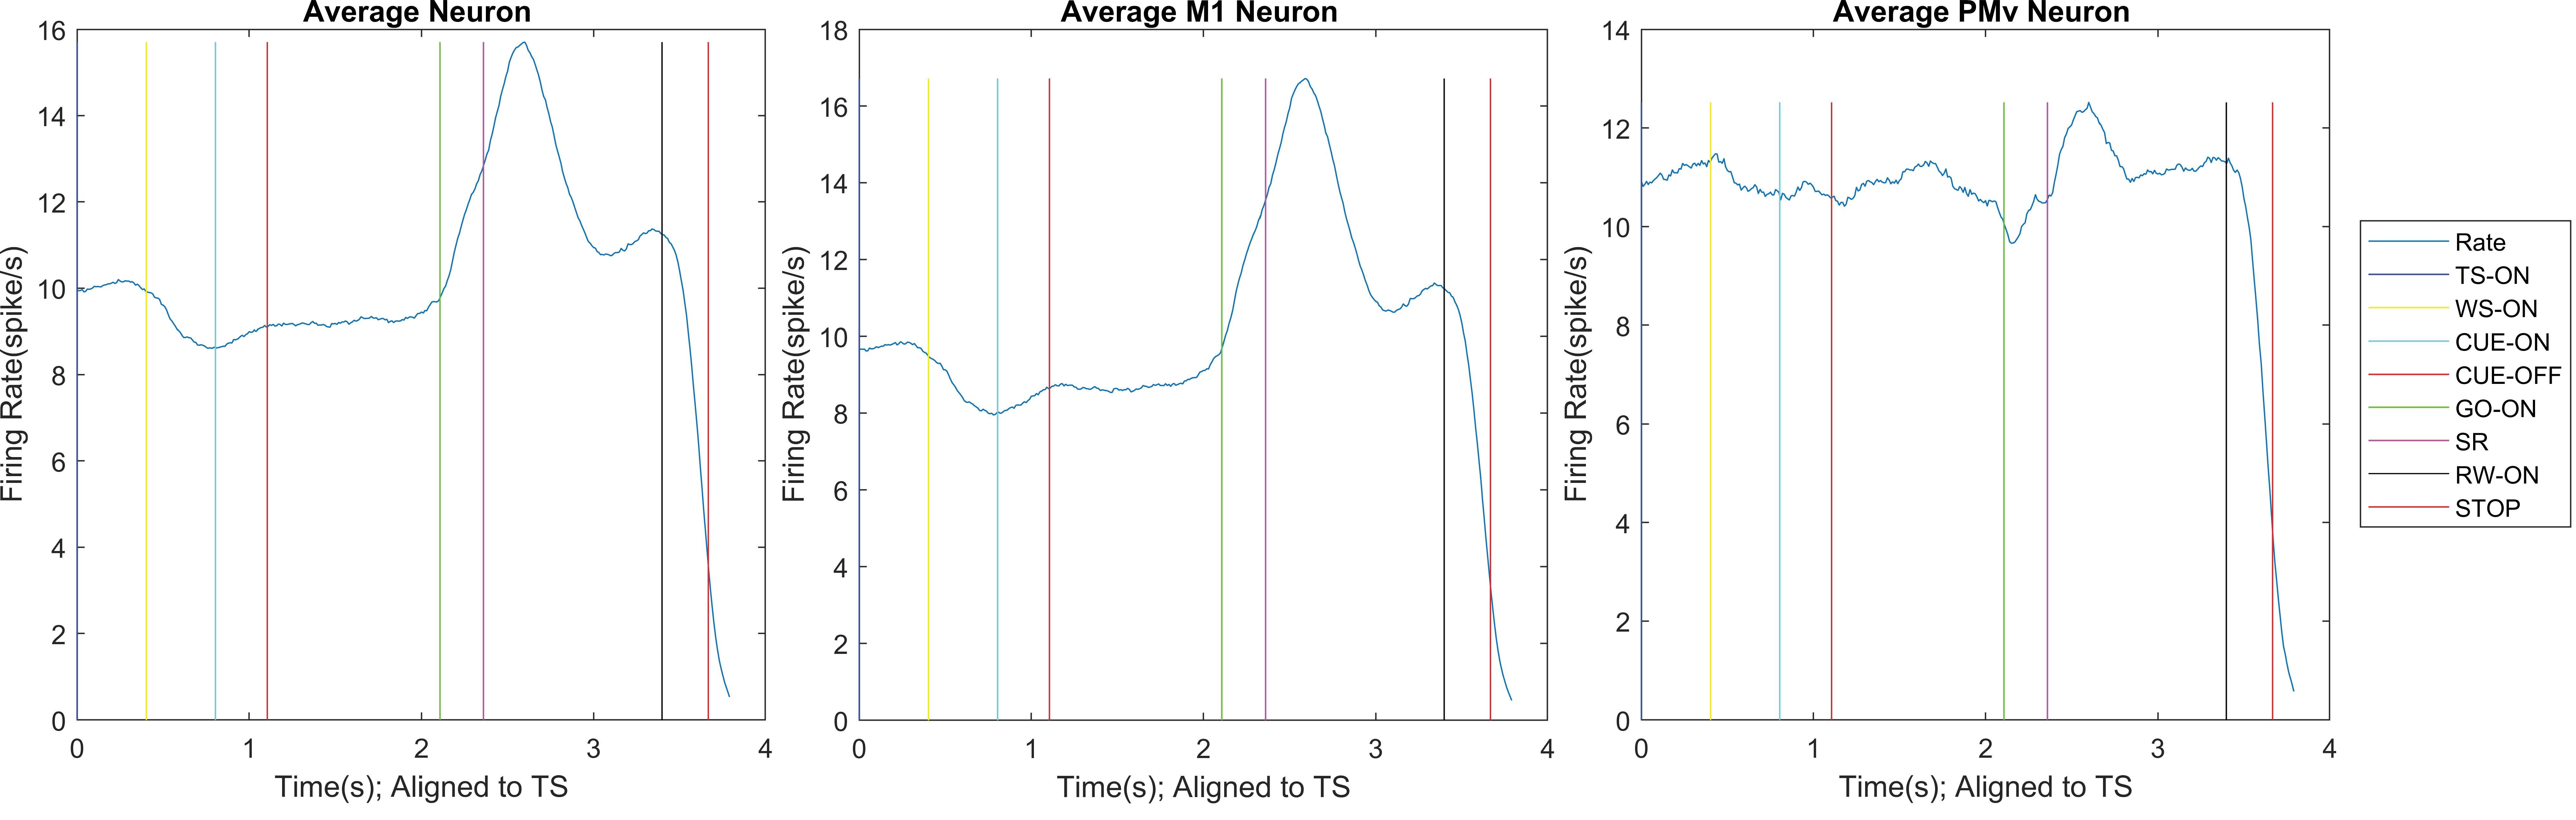
\includegraphics[width=11.4cm]{fig7.jpg}
\caption{Average PSTH plots. These plots show the average PSTH plots of: all neurons, M1 neurons, and PMv neurons respectively}\label{fig:side}
\end{SCfigure*}
\\
From the observation we had in the average PSTH plots, we hypothesize that the average neuron has a significant firing increase after the SR event. To test this assumption, we have to gather sufficient data from our desired variable, which is the firing rate, both for before (Null hypo.) and after (Alternate hypo.) the SR event. For each trial, we calculated the average firing rates on all neurons in two equal timing windows before and after SR, in a manner that our windows wouldn’t overlap with other events; especially with GO-ON. Subsequently, we were left with two firing rate distributions, collected from our trial range. These distributions that are shown in the figure below seem to have a near Gaussian distribution, which is expected from a large number average variable distribution. After running a T test with its predefined function in MATLAB, we calculated the p value indicating the probability of the difference between these two distributions being a zero mean Gaussian. The result showed the p value to be 1.18e-66 that is very smaller than the required threshold (0.01), and rejects our Null hypothesis. Additionally, we performed the same analysis regarding the GO-ON event and the result had a p value of 1.0e-49 which distinctly less than the latter recorded value. The conclusion of this investigation is that the firing rate is most sensitive to the SR event and the neural responses have a temporal correlation with this event which leads to the firing rate increase.\\
\begin{figure}%[tbhp]
\centering
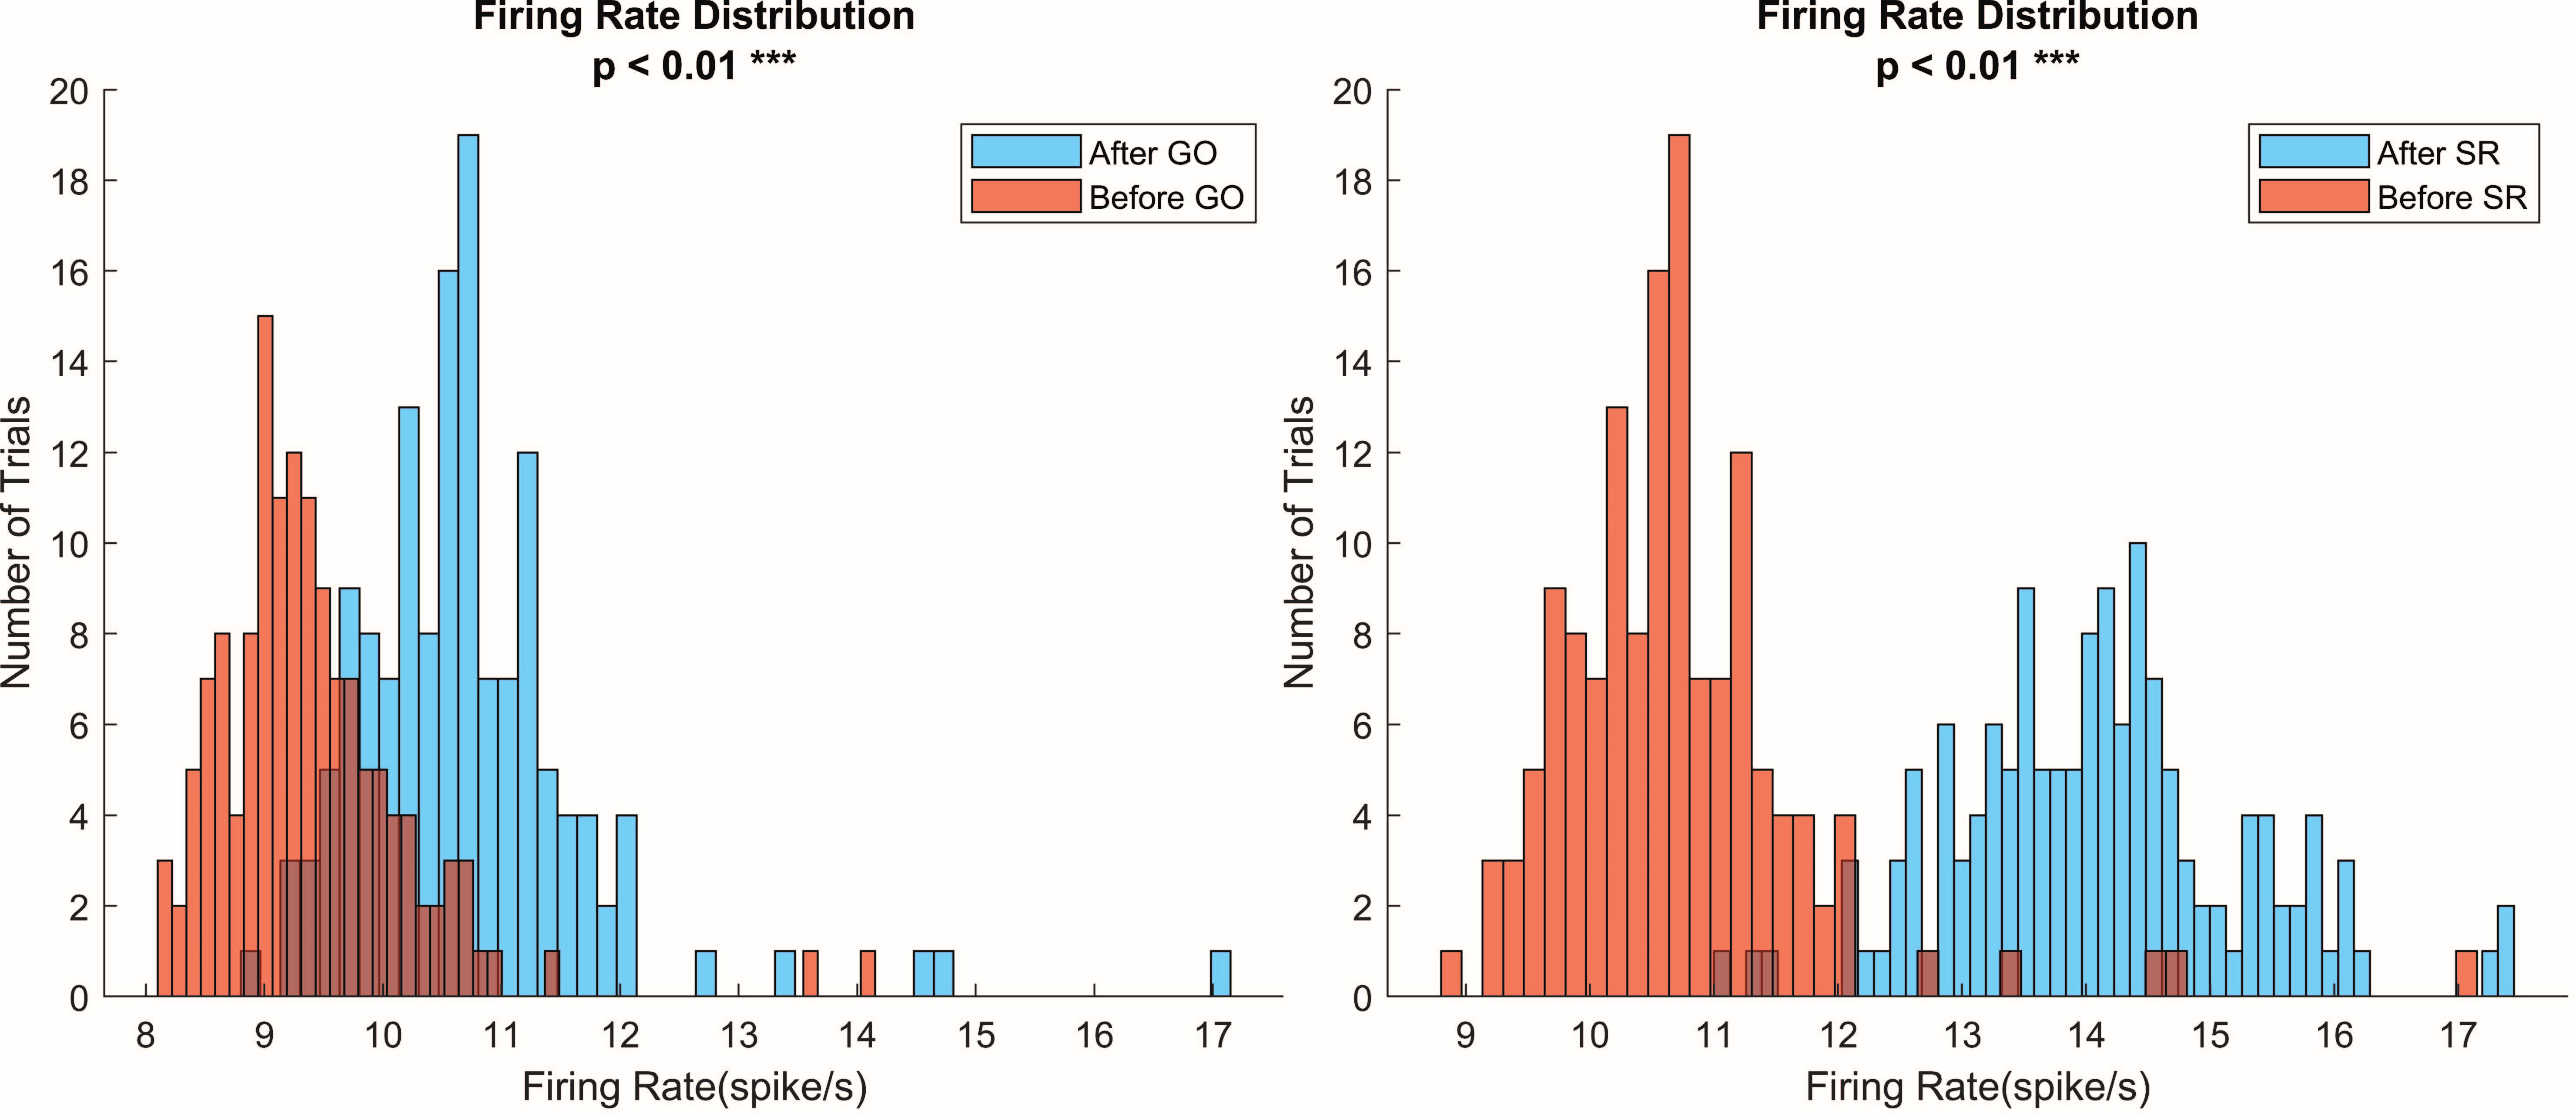
\includegraphics[width=.8\linewidth]{fig8.jpg}
\caption{Firing rate distributions. These pictures show the histogram of average firing rate distributions on the range of correct trials, both before and after a specific event; in our case: SR and GO-ON.}
\label{fig:frog}
\end{figure}
\\
Another statistical feature for comparing the firing patterns regarding an event is the Fano factor, which is calculated by dividing the variance of spike counts to its mean. We also measured this parameter on all neurons, before and after the SR event, which gave us two other Gaussian distributions on the range of trials. These distributions, as depicted in the next figure, have different means and a T test provided on these two, resulted in a p value of 4.6e-29 which shows the change of spike patterns after the SR event.
\\
\begin{figure}%[tbhp]
\centering
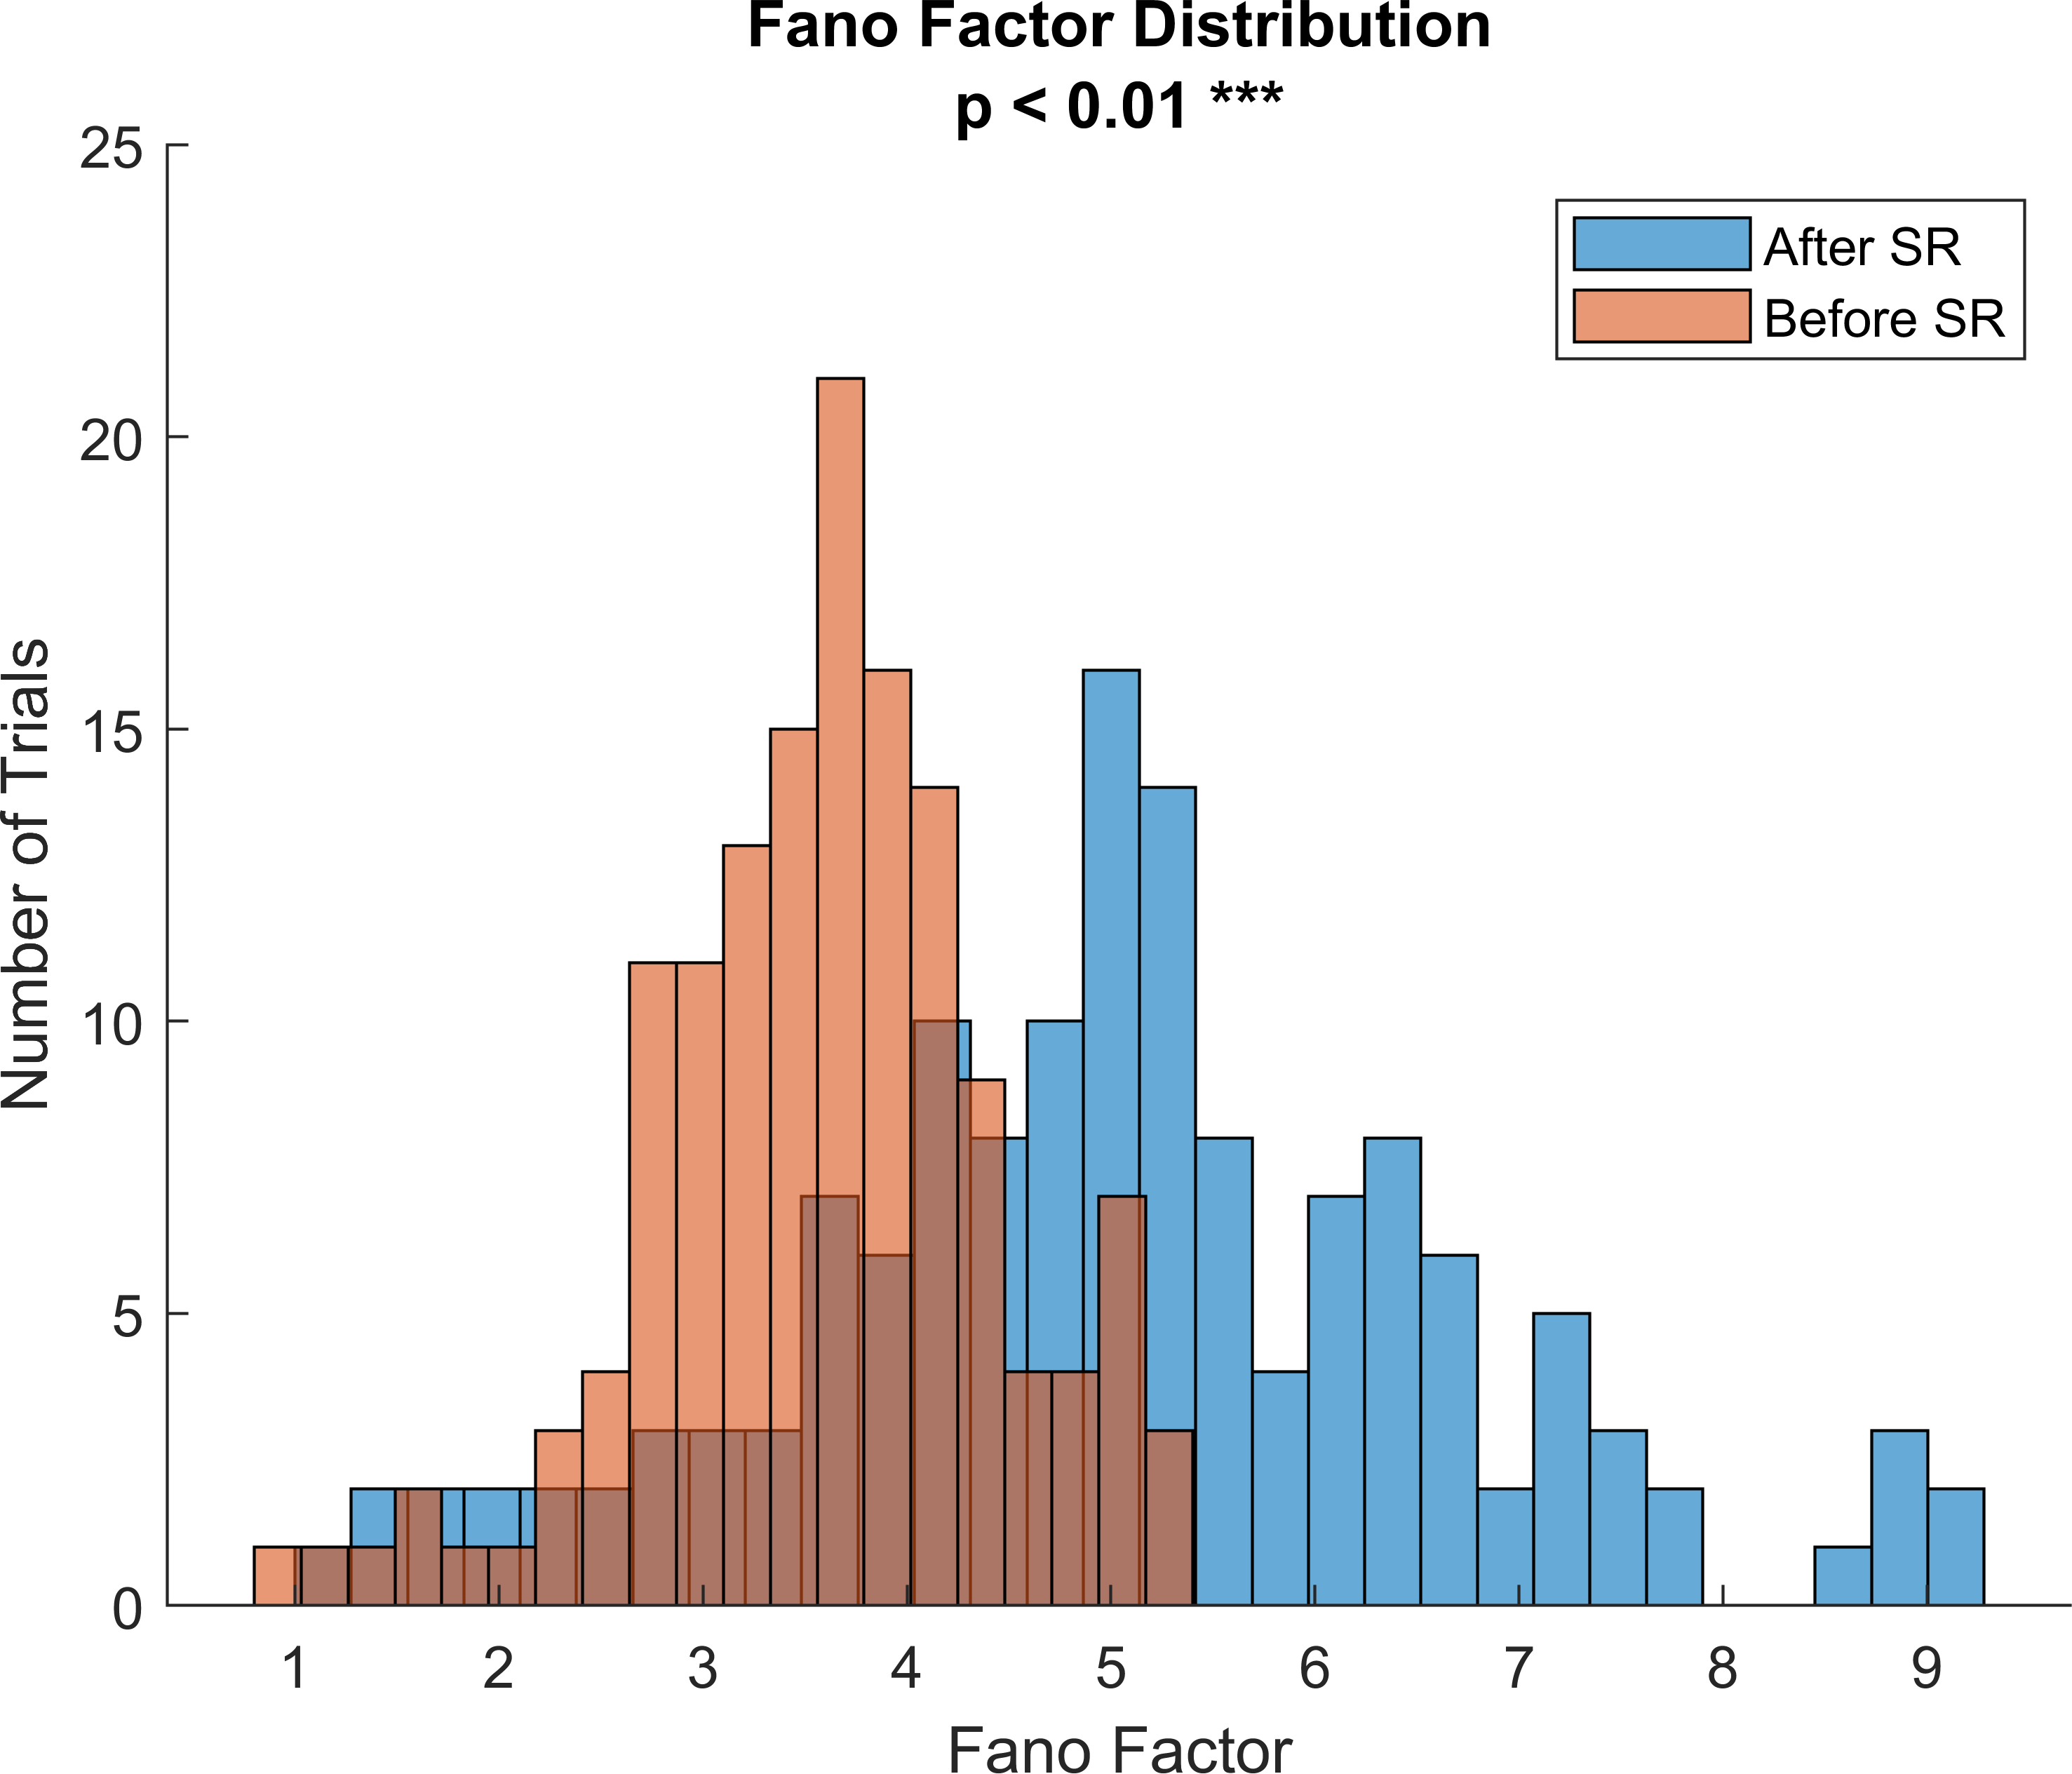
\includegraphics[width=.8\linewidth]{fig9.png}
\caption{Fano factor distribution. This picture shows the average Fano factor distribution both before and after SR.}
\label{fig:frog}
\end{figure}
\\
Another approach in this paper is to investigate the coding of specific neurons to various movement parameters such as direction and force. As we have previously mentioned, the dataset that we are working on has provided recordings for four different tasks and we managed to separate the trials associated with each of these four tasks. A simple method for distinguishing between neural responses in these tasks is to examine their PSTH plots. At first we went on extracting the average PSTH plots for each tasks, for which the results are shown in Fig. 9. But in these plots we didn’t discover any different patterns, probably because of the fact that we were gathering average information on all neurons and an average neuron might be doing a similar function in all tasks. But in our further analysis, we examined neurons individually. Although there were still many neurons with similar responses in all the four tasks, but we managed to find a rather significant amount of neurons which responded distinctively different to the direction-wise separated tasks. As shown in Fig. 10, some neurons responded with increased firing rates in PG tasks in contrast to SG tasks and some others in the reverse order. However, there wasn’t any significant response difference regarding force-related tasks. This may indicate that there are certain neurons playing a role in direction control, but it doesn’t seem likely for these neurons to be coding force related parameters.\\
\begin{figure}%[tbhp]
\centering
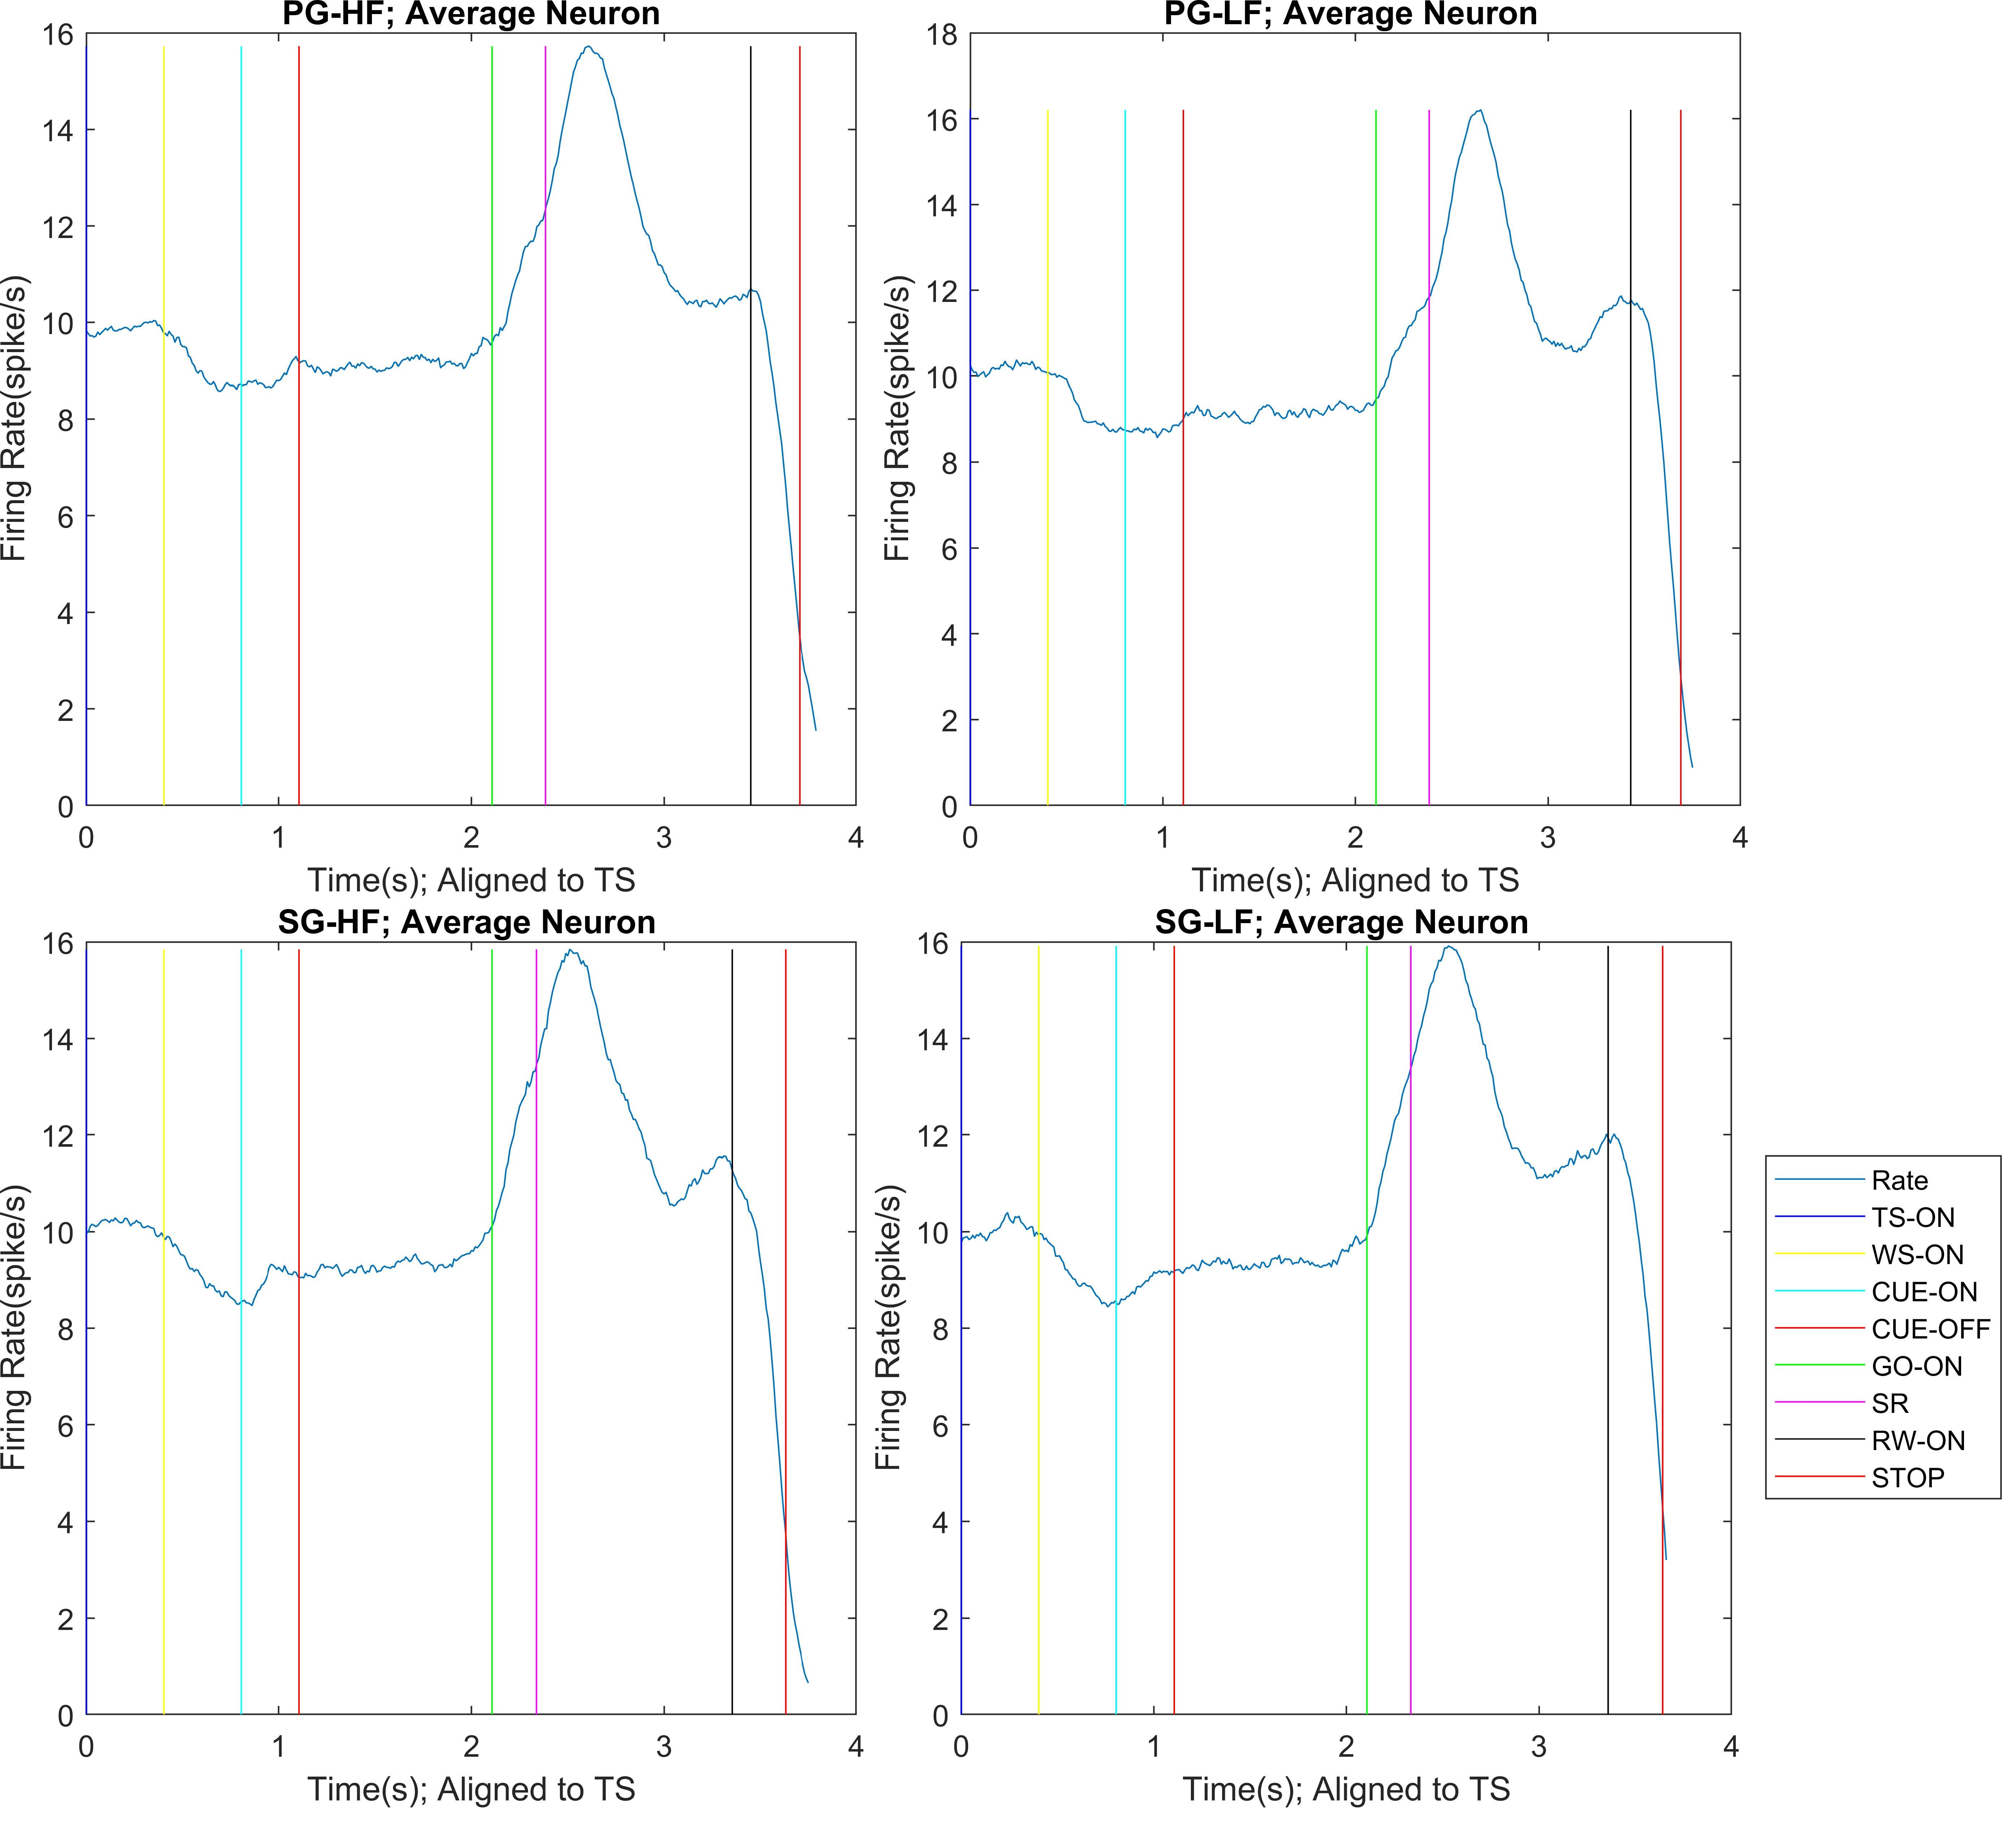
\includegraphics[width=.8\linewidth]{fig10.jpg}
\caption{Average PSTH of all four tasks. These four plots are collected by averaging the firing rates on all neurons, separated on the four different tasks.}
\label{fig:frog}
\end{figure}
\\
\begin{SCfigure*}[\sidecaptionrelwidth][t]
\centering
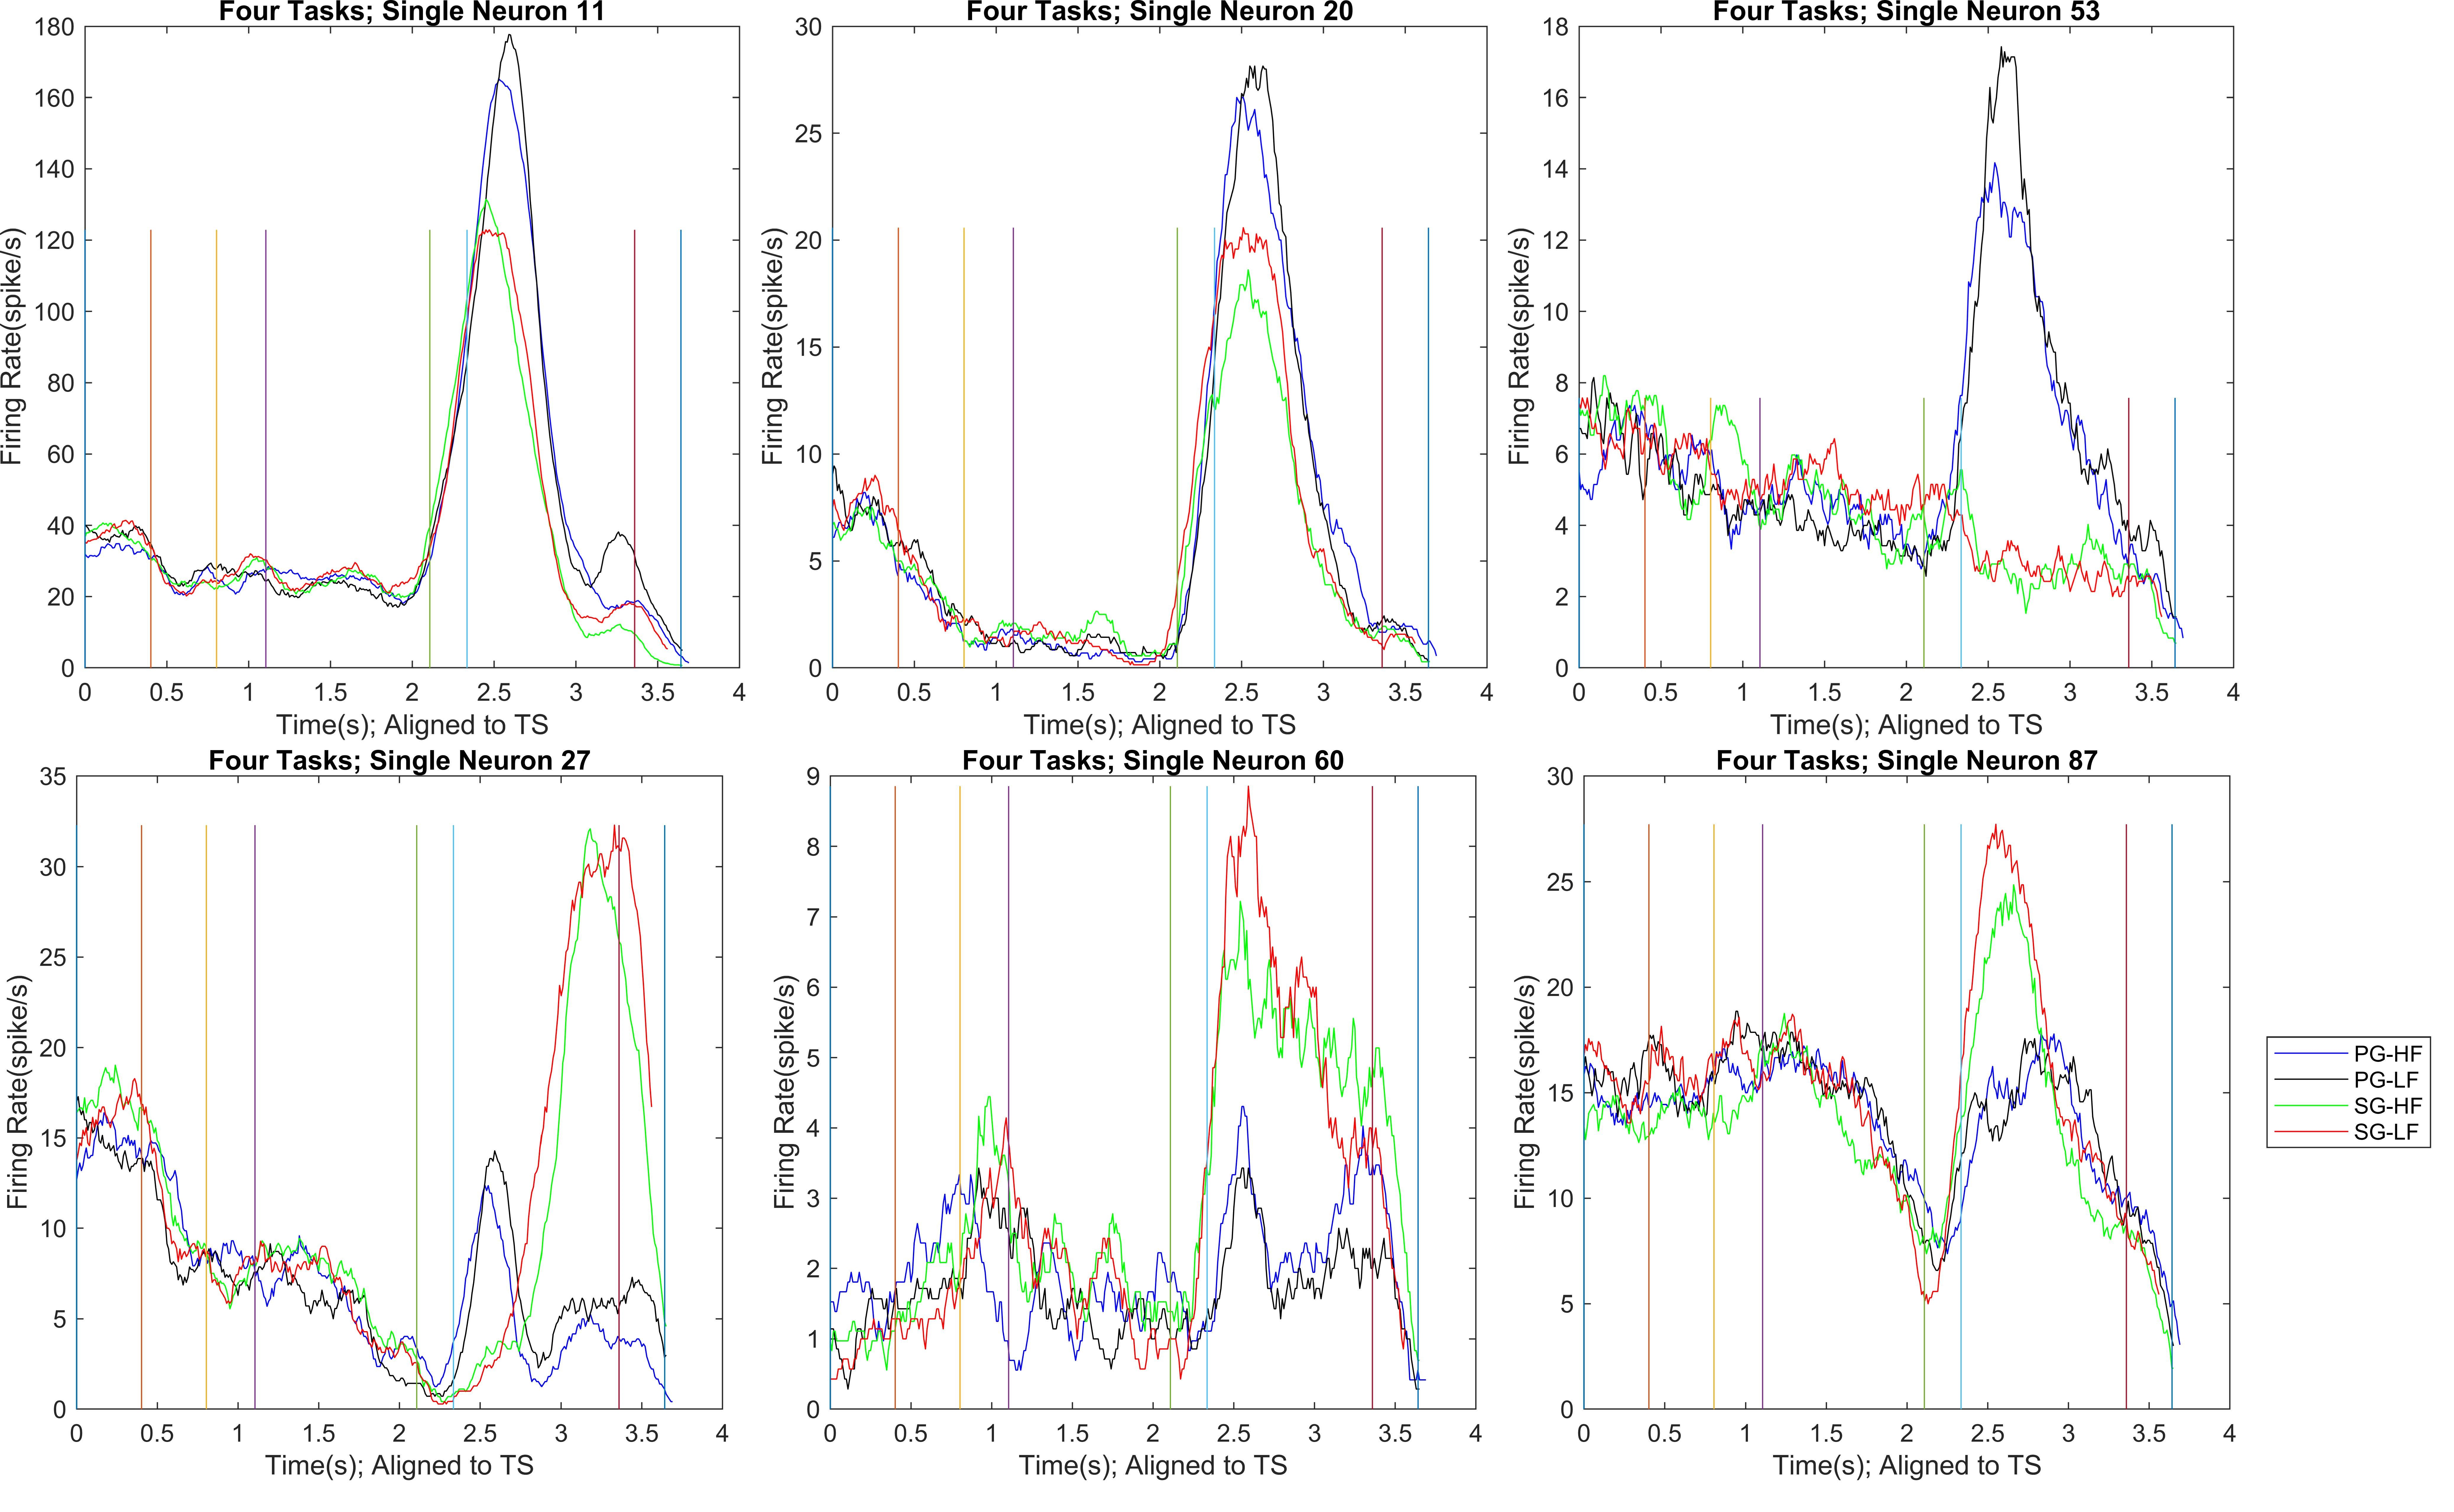
\includegraphics[width=11.4cm]{fig11.jpg}
\caption{Single neuron PSTH of four tasks. In these pictures the average firing rate for all the four tasks are shown in the same plot for each neuron (with four different colors). In three of the neurons we can see the significance of PG tasks, however in the other three, the SG tasks have more responses. Note that these neurons have been chosen from both area clusters, M1 and PMv..}\label{fig:side}
\end{SCfigure*}
\section*{Discussion}
In this paper we went on to show the positive correlation between the initiation of hand movement (shown by SR event), and temporal neural response in a reach-to-grasp activity; In other words, the near time occurrence of firing rate increase and the SR. We also managed to identify a number of neurons that responded differently to direction specific tasks, but we couldn’t find evidence regarding the response difference of force specific tasks.
\\
The relevance between of movement direction and neural response has been detected in previous experiments by performing center-out-reaching tasks (Georgopoulos et al. 1982; Schwartz et al. 1988). And there has been evidence that neural responses tend to code movement parameters such as direction, that have similar results to the experiments we conducted in this paper. But we failed to examine all the direction or force related responses statistically.
\\
The results found in our research can open a new window to neural behavior and control in hand movements that is known to be one of the complex body gestures in primates. Future researches can provide more detailed and feature-specific tasks alongside with high resolution electrophysiological recordings accompanied by more intense statistical analysis in hope of a better understanding of hand-related motor activities.

\acknow{We thank Dr. Ghazizadeh and teacher assistants for defining this project and managing this university course.}

\showacknow{} % Display the acknowledgments section

\section*{References}
1. Mark M. Churchland and Krishna V. Shenoy, Temporal Complexity and Heterogeneity of Single-Neuron Activity in Premotor and Motor Cortex, 2007
\\
2. Thomas Brochier, Massively parallel recordings in macaque motor cortex during an instructed delayed reach-to-grasp task, 2018

\end{document}